\documentclass[../main.tex]{subfiles}

\begin{document}

\section{Overwiew}
\label{section:problem:overview}

\begin{figure}[h]
    \centering
    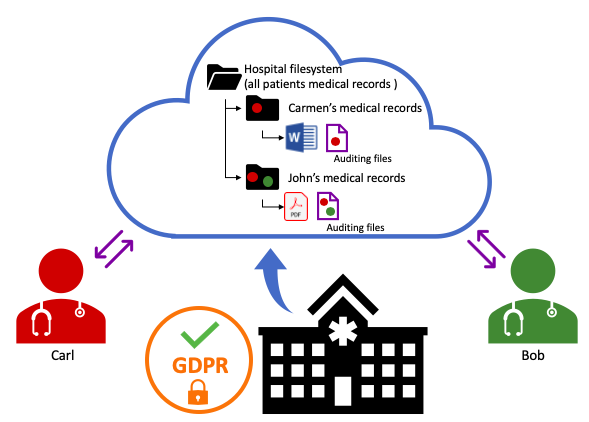
\includegraphics[width=0.75\textwidth]{images/problem/overview}
    
    \caption{Representation of the real life situation}
    \label{figure:problem:overview}
\end{figure}

\par To motivate our work, we are using an example linked to the healthcare domain, more precisely the hospitals. Inside a hospital, many services or doctors must share medical records of a single patient, as depicted in Figure \ref{figure:problem:overview}. How can those parties share this record without disclosing its content (to other parties) and without requiring complicated operation? On top of that, the revocation of a doctor right to access a specific resource, once he no longer needs it, is also a mandatory operation according to GDPR.

\medbreak
\par Alongside data confidentiality, keeping track of who accessed or edited a given file is required. GDPR states that: "\textit{All EU institutions have the legal obligation to keep a central register of records of activities processing personal data}". In practice, this means that every time an authorised doctor wants to access a medical record, s/he must first explain its intention. These intents explain the purpose of the action. These purposes allow a data owner (e.g: a patient) to know who accessed his information and avoid allowed users from abusing his private data. As the purpose may itself contain confidential information, it must also be securely stored. Most of all, these intents can not be tampered with, to keep their accuracy. Furthermore, for a forensic purpose, it would also be interesting to spot if unauthorised users are trying to alter these data. To top it all, these intents must be easily accessible for GDPR compliance evidence.

\medbreak
\par Aside from the two above functionalities, it is important to note that the users may use portable devices that works entirely offline whereas the concerned user must have a copy of the required documents (e.g: in the event of an out-of-the-office consultation in a remote area whereas there is very poor connectivity or even no internet at all). Furthermore, users must still be able to use their conventional legacy applications (e.g: such as PDF Reader, Microsoft Word, etc) as forcing them to use a new application is difficult and incurs a lot of extra work to the users. We wish to bring no extra complication to the end-users, they should barely see the difference compared to a standard filesystem.

\end{document}